\section{Transformationen}
\label{sec:Kap-9.3}

\vspace{2mm} %%% für Druck

Während man die Klassen, die man in UML-Klassendiagrammen modelliert hat, durch Programmiersprachenelemente ausdrücken und so auch ihre modellierten Attri\-bute und Operationen direkt in Programmcode übertragen kann, ist das für die Assoziationen eines Klassendiagramms nicht unmittelbar möglich. Objektorien\-tierte Programmiersprachen bieten kein direktes Element „Assoziation“ an. Entwickler müssen daher überlegen, durch welche Kombinationen und Konstruktionen der Programmier\-sprachen-Elemente die UML-Assoziationen umgesetzt werden können. Für diese sogenannten \textit{Transformationen} gibt es aus Erfahrungswissen entstandene Heuristiken, die sicher nicht in jedem Einzelfall die perfekte Lösung bieten, aber im Allgemeinen gangbare Wege aufzeigen. Üblicherweise finden die Transformationen noch auf UML-Ebene statt, und erst das Ergebnis der Transformation wird in den Quellcode der Zielsprache umgesetzt. Man transformiert also zunächst ein UML-Modell in ein anderes und kann letzteres dann direkt in Elemente der Programmier\-sprache umsetzen (bzw. automatisiert umsetzen lassen). Für erfahrene Entwickler ist es durchaus auch möglich, sich den expliziten Transformationsschritt auf UML-Ebene zu sparen, die Transformationen nur implizit „im Kopf“ vorzunehmen und direkt den entsprechenden Quellcode zu schreiben. Insbesondere in Projekten, die die Software\-engineering\-prozesse des Entwurfs und der Implementierung eng verzahnen, wird man in der Regel auf die zusätzliche UML-Modellebene verzichten.

\vspace{2mm} %%% für Druck

Assoziationen werden durch die Eigenschaften Navigierbarkeit und Multiplizität charakterisiert, so dass man vor der Anwendung einer Transformation folgende Fragen klären muss:

\vspace{2mm} %%% für Druck

\begin{itemize}
	\item Ist die Navigierbarkeit einseitig oder bidirektional?
	\vspace{2mm} %%% für Druck
	\item Sind die Multiplizitäten der beiden Assoziationsenden beschränkt (\zb \sttpUMLText{0..2}), exakt (\zb \sttpUMLText{1}) oder unbeschränkt (\sttpUMLText{*})?
\end{itemize}

\vspace{2mm} %%% für Druck

Wir beginnen mit der Transformation einseitig navigierbarer 1-zu-1-Assoziationen (im Folgenden verkürzt geschrieben als 1:1-Assoziation) und führen dann die Transformation komplexerer Assoziationen darauf zurück.

\clearpage %%% für Druck

\minisec{Einseitig navigierbare 1:1-Assoziationen}

\vspace{2mm} %%% für Druck

In diesem, einfachsten Fall kann man die Assoziation direkt auf ein neu zu deklarierendes Attribut der Klasse transformieren, von der aus die Assoziation navigierbar ist. Das Attribut erhält den Namen der Assoziation oder den der Rolle der assoziierten Klasse. Abbildung~\ref{fig:transformationen_abb_a} zeigt ein Beispiel.

\vspace{2mm} %%% für Druck

Eine Klasse \sttpUMLText{Professor} und eine Klasse \sttpUMLText{Raum} sind über eine einseitig navigierbare (von \sttpUMLText{Professor} zu \sttpUMLText{Raum}) Assoziation verbunden. Diese Assoziation kann transformiert werden, indem der Klasse \sttpUMLText{Professor} ein Attribut \sttpUMLText{dienstzimmer} hinzugefügt wird. In diesem Attribut wird der Raum gespeichert, der als Dienstzimmer des Profes\-sors fungiert, programmierspachlich: das Attribut \sttpUMLText{dienstzimmer} hat den Daten\-typ \sttpUMLText{Raum}. Gleichzeitig wird noch ein Mechanismus benötigt, wie die Zuordnung einer Instanz der Klasse \sttpUMLText{Raum} zu einer Instanz der Klasse \sttpUMLText{Professor} vorgenommen und auch wieder gelöst werden kann. Das kann zum Beispiel über zwei entsprechend gestaltete Operationen \sttpUMLText{verbinde} und \sttpUMLText{löse} in der Klasse \sttpUMLText{Professor} erfolgen.

\begin{figure}[h!]
	\centering
	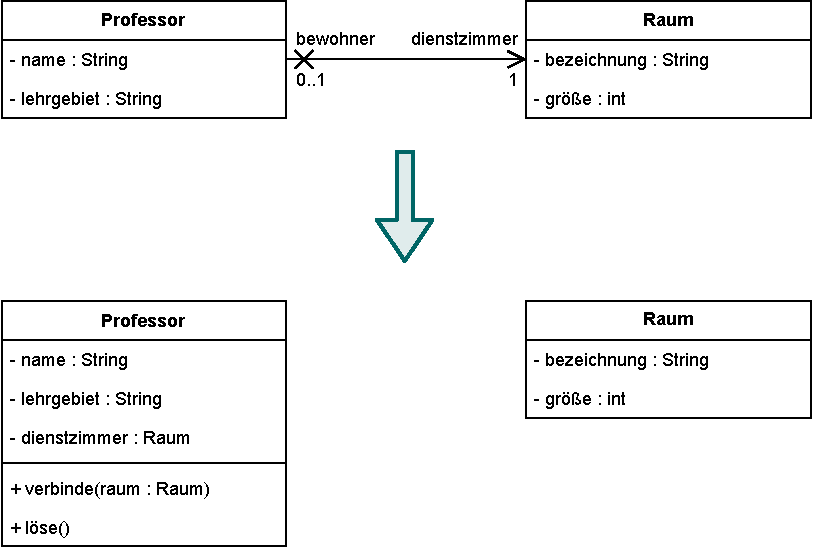
\includegraphics[scale=1.0]{Bilder/Kapitel-9/transformationen_abb_a.pdf}
	\vspace{\baselineskip} %%% für Druck
	\caption{Transformation einer einseitig navigierbaren 1:1-Assoziation}
	\label{fig:transformationen_abb_a}
\end{figure}

\pagebreak %%% für Druck

\minisec{Bidirektional navigierbare 1:1-Assoziationen}

\vspace{2mm} %%% für Druck

Bidirektional navigierbare 1:1-Assoziationen transformiert man auf je ein Attribut in beiden an der Assoziation beteiligten Klassen. Die Konsistenz der Verbindungen, \zb dass bei dem Aufbau einer Verbindung die Attribute in beiden Instanzen mit den richtigen verbundenen Instanzen (Referenzen) besetzt werden, muss durch entsprechende Operationen zum Verbinden und zum Lösen der Verbindung sichergestellt werden. Zum Beispiel darf eine Verbindung nur dann eingegangen werden, wenn ein Objekt nicht bereits verbunden ist.

\vspace{2mm} %%% für Druck

Abbildung~\ref{fig:transformationen_abb_b} zeigt wieder das Beispiel mit den Klassen \sttpUMLText{Professor} und \sttpUMLText{Raum}. Diesmal soll es sich jedoch um eine bidirektional navigierbare Assoziation handeln, also Instanzen der Klasse \sttpUMLText{Raum} kennen, im Unterschied zu Abbildung~\ref{fig:transformationen_abb_a} auch Instanzen der Klasse \sttpUMLText{Professor}.

\begin{figure}[h!]
	\centering
	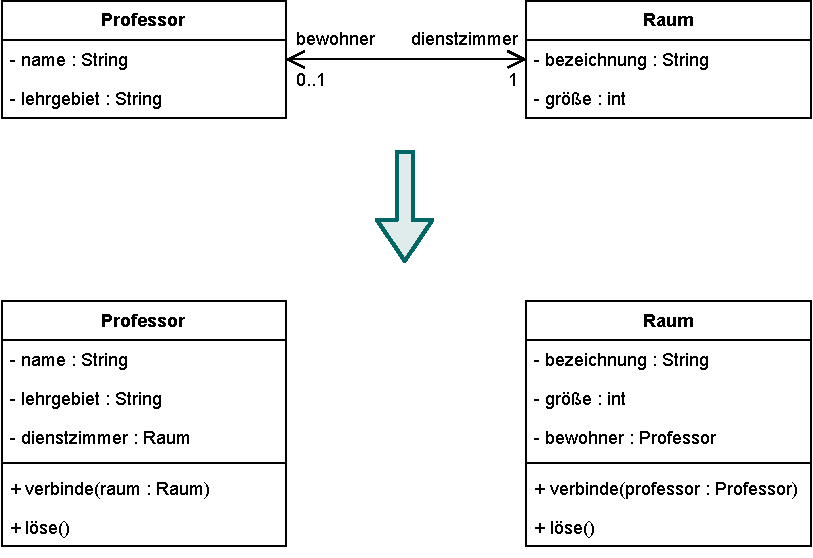
\includegraphics[scale=1.0]{Bilder/Kapitel-9/transformationen_abb_b.pdf}
	\vspace{\baselineskip} %%% für Druck
	\caption{Transformation einer bidirektional navigierbaren 1:1-Assoziation}
	\label{fig:transformationen_abb_b}
\end{figure}

\pagebreak %%% für Druck

\minisec{Einseitig navigierbare 1:n-Assoziationen mit festem n}

\vspace{2mm} %%% für Druck

Zunächst betrachten wir 1:n-Assoziationen mit \textbf{festem und sehr kleinem n}. In solchen Fällen können wir für jede Referenz ein Attribut vorsehen.

\vspace{2mm} %%% für Druck

Abbildung~\ref{fig:transformationen_abb_c} zeigt eine einseitig navigierbare Assoziation zwischen den Klassen \sttpUMLText{Strecke} und \sttpUMLText{Punkt}, am \sttpUMLText{Punkt}-Ende eine Multiplizität von exakt \sttpUMLText{2}, \dasHeisst jeder Instanz der Klasse \sttpUMLText{Strecke} sind immer genau zwei Instanzen der Klasse \sttpUMLText{Punkt} zugeordnet. Bei der Transformation erhält die Klasse \sttpUMLText{Strecke} jetzt genau zwei Attribute, in denen diese \sttpUMLText{Punkt}-Instanzen gespeichert werden. Das Prinzip ist identisch zum Beispiel aus Abbildung~\ref{fig:transformationen_abb_a}.

\begin{figure}[h!]
	\centering
	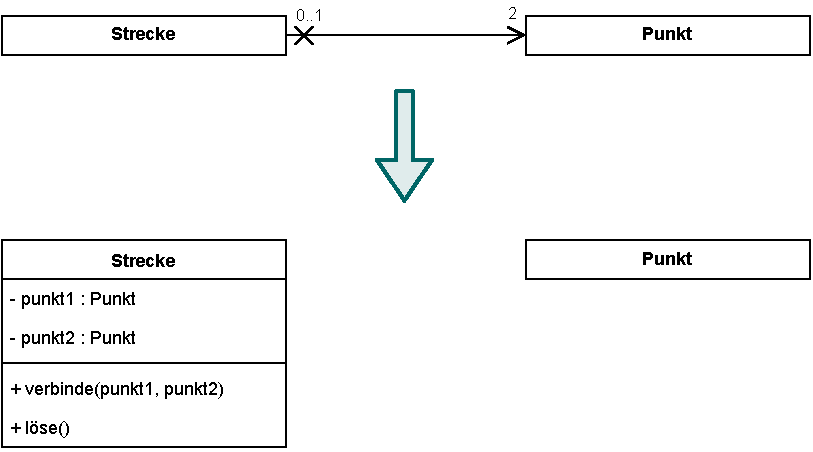
\includegraphics[scale=1.0]{Bilder/Kapitel-9/transformationen_abb_c.pdf}
	\vspace{\baselineskip} %%% für Druck
	\caption{Transformation einer 1:n Assoziation mit n = 2}
	\label{fig:transformationen_abb_c}
\end{figure}

\pagebreak %%% für Druck

\minisec{~~~} % leere Überschrift, damit Text mit demselben Abstand von oben beginnt wie auf der vorherigen Seite
\vspace{2mm} %%% für Druck

Bei 1:n-Assoziationen mit \textbf{festem und großem n} können die Referenzen auf verbundene Instanzen auch in einem Feld (in Java: Array) vorgehalten werden. Abbildung~\ref{fig:transformationen_abb_d} zeigt einen solchen Fall.

\vspace{2mm} %%% für Druck

Im Modell einer Kabinenschwebebahn besteht von der Klasse \sttpUMLText{Kabine} eine einseitig navigierbare Assoziation zu der Klasse \sttpUMLText{Person}, wobei in einer Kabine bis zu 20 Personen transportiert werden können. Bei der Transformation der Klasse \sttpUMLText{Kabine} wird das Attribut \sttpUMLText{personen} vom Array-Typ \sttpUMLText{Person[20]} für die verbundenen Personeninstanzen vorgesehen.

\begin{figure}[h!]
	\centering
	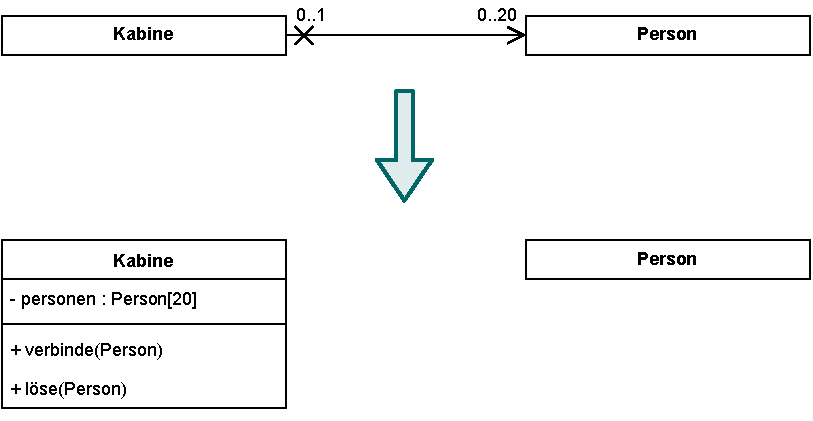
\includegraphics[scale=1.0]{Bilder/Kapitel-9/transformationen_abb_d.pdf}
	\vspace{\baselineskip} %%% für Druck
	\caption{Assoziation mit unidirektionaler Navigierbarkeit und beschränkter Multiplizität}
	\label{fig:transformationen_abb_d}
\end{figure}

\pagebreak %%% für Druck

\minisec{Einseitig navigierbare 1:n-Assoziationen mit variablem n}

\vspace{2mm} %%% für Druck

Bei 1:n-Assoziationen mit variabler oberer Grenze der Multiplizität hängt die Transformation wesentlich von der Richtung der Navigierbarkeit ab. Ist die Assoziation zu der Klasse hin navigierbar, von der höchstens eine Instanz an einer entsprechenden Verbindung teilnimmt, reicht die für einseitig navigierbare 1:1-Assoziationen vorgestellte Transformation aus. Im umgekehrten Fall müssen bezüglich der Assoziation mehrere verbundene Instanzen (tatsächlich deren Referenzen) gespeichert werden. Dies führen wir auf eine 1:1-Assoziation zu einer Behälterklasse zurück, die eine Menge von Objekten aufnehmen kann. Als Behälterklasse wählt man \zb in Java eine Unterklasse einer entsprechenden Bibliotheksklasse bzw. realisiert ein Interface wie Collection, Set oder List.

\vspace{2mm} %%% für Druck

Wir untersuchen die Unterschiede anhand der in der oberen Hälfte von Abbildung~\ref{fig:transformationen_abb_e} dargestellten 1:n-Assoziation zwischen \sttpUMLText{Restaurant} und \sttpUMLText{Person}. Ist die Navigation von der Klasse \sttpUMLText{Person} zur Klasse \sttpUMLText{Restaurant} vorgesehen, so muss die Klasse \sttpUMLText{Person} lediglich mit einem Attribut \sttpUMLText{stammlokal} ausgestattet werden, welches (die Referenz auf) die verbundene Restaurantinstanz aufnimmt.

\begin{figure}[h!]
	\centering
	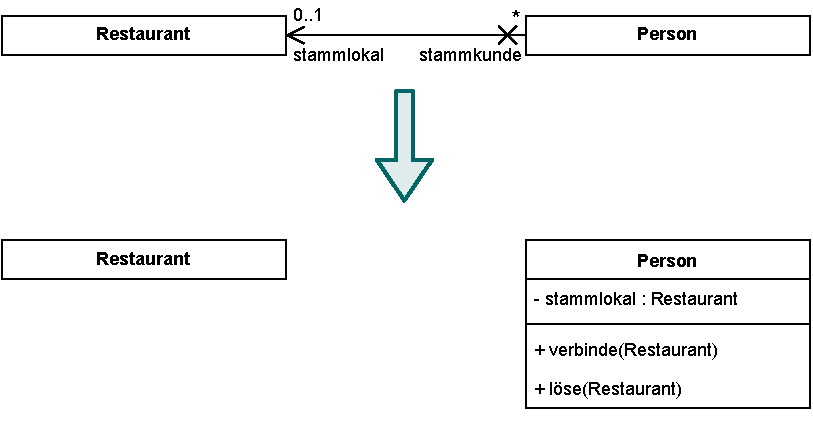
\includegraphics[scale=1.0]{Bilder/Kapitel-9/transformationen_abb_e.pdf}
	\vspace{\baselineskip} %%% für Druck
	\caption{Transformation einer 1:n-Assoziation mit variablem n und Navigierbarkeit in Richtung der Multiplizität 0..1}
	\label{fig:transformationen_abb_e}
\end{figure}

\pagebreak %%% für Druck

\minisec{~~~} % leere Überschrift, damit Text mit demselben Abstand von oben beginnt wie auf der vorherigen Seite
\vspace{2mm} %%% für Druck

Bei umgekehrter Navigationsrichtung müssen wir in einer Restaurantinstanz mehrere Referenzen zu Personeninstanzen nachhalten. Hierzu führen wir eine Behälterklasse \sttpUMLText{StammkundeMenge} (\zb als Unterklasse einer das Interface Set realisierenden Bibliotheks\-klasse wie \sttpUMLText{HashSet} oder \sttpUMLText{TreeSet}) ein, zu der die Klasse \sttpUMLText{Restaurant} in einer Komposition steht und die (Referenzen auf) mehrere Personeninstanzen speichern kann. Diese Vorgehensweise ist in Abbildung~\ref{fig:transformationen_abb_f} dargestellt.

\begin{figure}[h!]
	\centering
	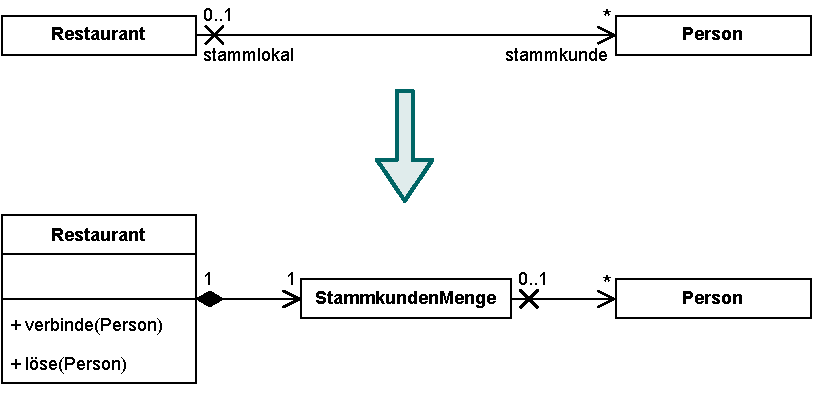
\includegraphics[scale=1.0]{Bilder/Kapitel-9/transformationen_abb_f.pdf}
	\vspace{\baselineskip} %%% für Druck
	\caption{Transformation einer 1:n-Assoziation mit Navigierbarkeit in Richtung der Multiplizität *}
	\label{fig:transformationen_abb_f}
\end{figure}

\pagebreak %%% für Druck

\minisec{Bidirektional navigierbare 1:n-Assoziationen}

\vspace{2mm} %%% für Druck

Ist die bidirektionale Navigierbarkeit einer 1:n-Assoziation erforderlich, spalten wir diese in zwei einseitig navigierbare 1:n-Assoziationen auf, die wir jeweils wie oben beschrieben transformieren.

\vspace{2mm} %%% für Druck

In dem oberen Klassendiagramm in Abbildung~\ref{fig:transformationen_abb_g} ist die Assoziation zwischen den Klassen \sttpUMLText{Restaurant} und \sttpUMLText{Person} bidirektional navigierbar. Das untere Klassen\-diagramm zeigt die aus der Transformation resultierenden beiden einseitig navigierbaren 1:n-As\-so\-zi\-a\-ti\-o\-nen \sttpUMLText{Stammkunde} und \sttpUMLText{Stammlokal}. Diese müssten nun noch wie in Abbildung~\ref{fig:transformationen_abb_e} bzw. Abbildung~\ref{fig:transformationen_abb_f} dargestellt transformiert werden.

\begin{figure}[h!]
	\centering
	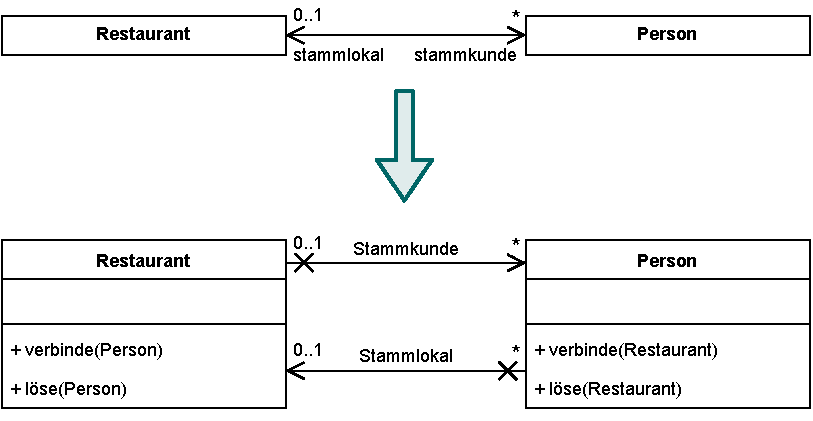
\includegraphics[scale=1.0]{Bilder/Kapitel-9/transformationen_abb_g.pdf}
	\vspace{\baselineskip} %%% für Druck
	\caption{Transformation einer 1:n-Assoziation mit bidirektionaler Navigierbarkeit}
	\label{fig:transformationen_abb_g}
\end{figure}

\pagebreak %%% für Druck

\minisec{Transformation von n:m-Assoziationen}

\vspace{2mm} %%% für Druck

Da n:m-Assoziationen in den meisten Fällen bidirektional navigierbar sind, betrachten wir nur diesen Fall. Die Transformation einer n:m-Assoziation beinhaltet zunächst das Hinzufügen einer weiteren Klasse, deren Instanzen (Referenzen auf) jeweils zwei miteinander verbundene Instanzen der assoziierten Klassen enthalten. Jede Instanz dieser Klasse stellt ein Paar dar — wir sprechen von der Paarklasse der (transformierten) n:m-Assoziation. Von der global sichtbaren einzigen Instanz einer Relationsklasse (hier wird das Entwurfsmuster Einzelstück (Singleton) verwendet) werden alle Paarinstanzen verwaltet und Iteratoren zum Zugriff auf die mit einer Instanz verbundenen Instanzen zur Verfügung gestellt. Instanzen der Paarklasse werden ausschließlich von der Instanz der Relationsklasse erzeugt. Abbildung~\ref{fig:transformationen_abb_h} zeigt ein Beispiel.

\begin{figure}[h!]
	\centering
	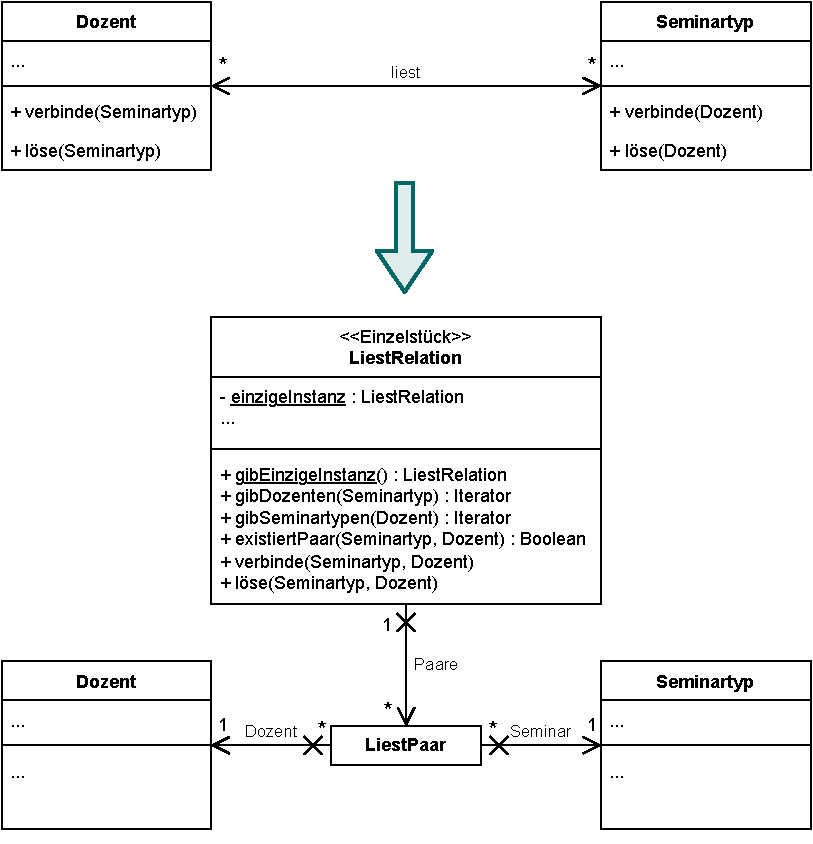
\includegraphics[scale=1.0]{Bilder/Kapitel-9/transformationen_abb_h.pdf}
	\vspace{\baselineskip} %%% für Druck
	\caption{Transformation einer n:m-Assoziation}
	\label{fig:transformationen_abb_h}
\end{figure}

\pagebreak %%% für Druck

Für die Assoziation zwischen den Klassen \sttpUMLText{Dozent} und \sttpUMLText{Seminartyp} besteht die Transformation aus Hinzufügen der Paarklasse \sttpUMLText{LiestPaar}, deren Instanzen Paare von Verweisen auf zwei verbundene Dozenten- und Seminartypobjekte enthalten (Abb.~\ref{fig:transformationen_abb_h}, unteres Diagramm). Die ebenfalls neu hinzugefügte Relationsklasse \sttpUMLText{LiestRelation} kennt alle Instanzen der Klasse \sttpUMLText{LiestPaar} und stellt Iteratoren zum Zugriff auf zugeordnete Instanzen der Klassen \sttpUMLText{Dozent} bzw. \sttpUMLText{Seminartyp} zur Verfügung.

\vspace{2mm} %%% für Druck

Die Operationen der Einzelstück-Klasse \sttpUMLText{LiestRelation} realisieren folgende Funktionen zur Verwaltung der \sttpUMLText{LiestPaar}-Instanzen:

\vspace{2mm} %%% für Druck

\begin{itemize}
	\item \sttpUMLText{gibDozenten(Seminartyp): Iterator} liefert einen Iterator, der alle Dozenten zu einem gegebenen Seminartyp durchläuft.
	\item \sttpUMLText{gibSeminartypen(Dozent): Iterator} liefert einen Iterator, der alle Seminar\-typen zu einem gegebenen Dozenten durchläuft.
	\item \sttpUMLText{existiertPaar(Seminartyp, Dozent): Boolean} prüft, ob die angegebene Verbindung existiert.
	\item \sttpUMLText{verbinde(Seminartyp, Dozent)} verbindet einen Seminartyp mit einem 
	\linebreak %%% für Druck
	Dozenten, indem eine \sttpUMLText{LiestPaar}-Instanz erzeugt und in die \sttpUMLText{LiestRelation} eingefügt wird. Die \sttpUMLText{LiestRelation}-Instanz überprüft, ob die Verbindung 
	\linebreak %%% für Druck
	zwischen dem Seminartyp und dem Dozenten nicht bereits besteht.
	\item \sttpUMLText{löse(Seminartyp, Dozent)} löst die angegebene Verbindung, sofern sie 
	\linebreak %%% für Druck
	besteht.
\end{itemize}